\chapter{Architectuur}\label{ch:Architectuur}

Om inzicht te verkrijgen in potentiële kwetsbaarheden in de projecten van Eaglescience moet er een applicatie worden ontworpen die in staat is om analyses uit te voeren op het moment dat er veranderingen worden aangebracht in deze projecten. Daarnaast moet de applicatie in staat zijn deze analyses uit te voeren op een periodieke basis.
Op het moment van schrijven wordt er binnen Eaglescience ontwikkeld in de talen Scala en NativeScript, maar de verwachting is dat er in de toekomst een mogelijkheid bestaat dat dit uitgebried gaat worden. Daarnaast is zijn deze twee talen niet de enige twee platformen binnen de stack, zo wordt er ook gebruik gemaakt van docker met daarbnij verschillende images die ook kwetsbaarheden kunnen bevatten. Dit ontwerp voorziet niet in de mogelijkheid om deze toekomstige platformen als ook docker te kunnen scannen. Het ontwerp moet wel zo zijn dat er een mogelijkheid bestaat om deze op een relatief makkelijke manier toe te voegen.

Analyses worden uitgevoerd op modulenniveau, hier zijn in basis twee redenen voor. Ten eerste is een module binnen een Eaglescience project een afgeschermd onderdeel dat een eigen platform benut. Ten tweede kan er op module niveau veranderingen worden verwacht ten opzichte van dependency declaraties.

In figuur~\ref{fig:SOUP-Components} is te zien welke componenten er nodig zijn om van informatie welke middels een Software Composition Tool(SCA) is verkregen te verwerken naar een rapport die in de portal te zien is. De verschillende componenten worden ieder in een eigen sectie uitvoerig besproken.%todo: nakijken na voltooien hoofdstuk
\begin{figure}[bth]
    \myfloatalign
    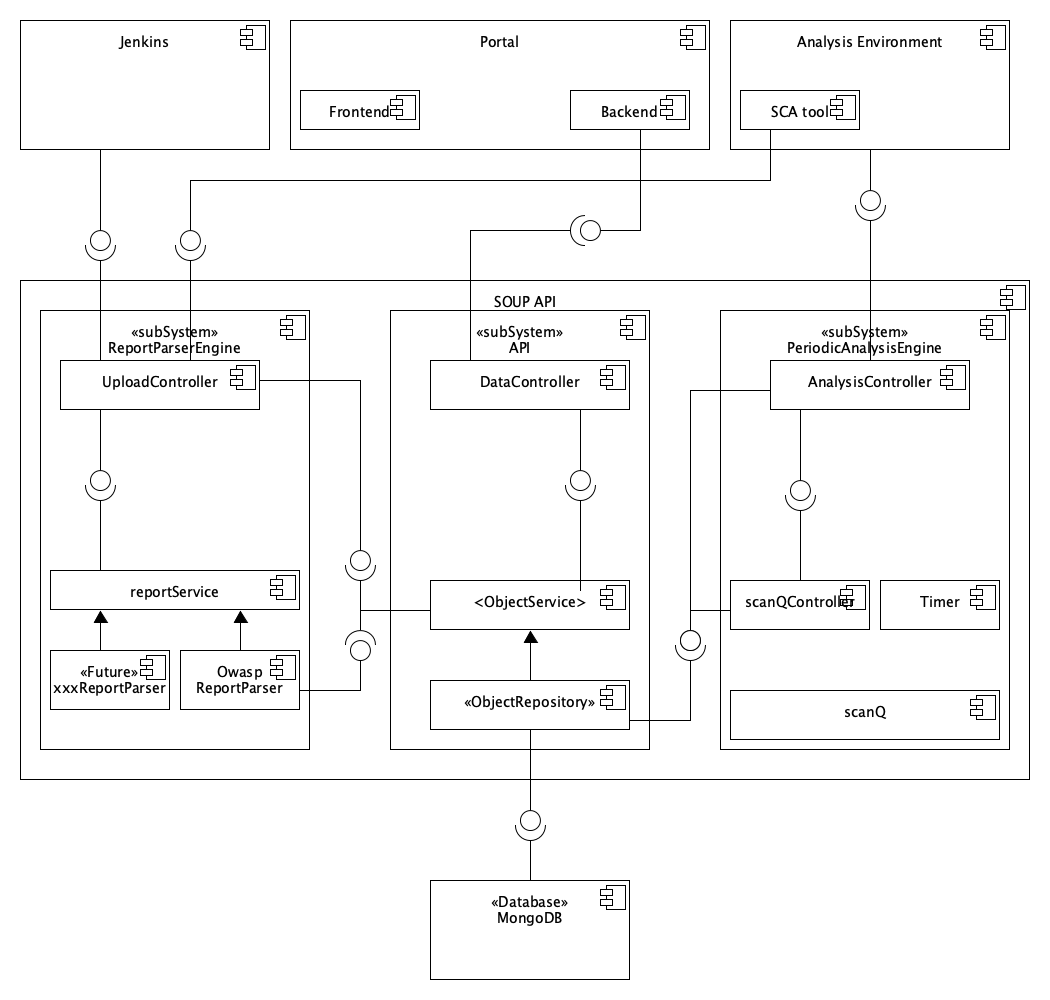
\includegraphics[width=10cm]{gfx/umlet/exports/ApplicationComponents}
    \caption{Componenten SOUP Analyse Systeem}
    \label{fig:SOUP-Components}
\end{figure}
    \section{Jenkins} De bestaande Jenkins omgeving wordt gebruikt voor de initiele analyses op modulen. Deze analyse wordt aangeboden aan de ReportParserEngine in de SOUPAPI. Het doet dit door eerst een analyse aan te vragen en vervolgens een Rapport en Dependency files te sturen.

Op het moment dat er in Jenkins een build wordt gedaan is er potientieel iets veranderd in de sourcecode en daarmee ook in de dependencies die er beschreven staan in de module. Door de SCA tooling hier al in te zetten kan er direct een rapport worden gegenereert die zichtbaar is in de portal. Hierdoor is er bijna direct inzicht in welke kwetsbaarheden er bekend zijn in het project. In de pipeline moet een onderdeel worden toegevoegd waardoor de SCA tooling kan worden uitgevoerd. Middels een BashScript dat een HTTP POST naar de SOUP API kan doen met daarin gegeven over de geanalyseerde module en het project. Eaglescience werkt met Tags om functionaliteiten binnen de pipeline te kunnen sturen het is wenselijk om hier een tag voor de soup analyse toe te voegen om eventueel de analyse uit te schakelen als dit wenselijk is.
    \section{Portal} De portal is een inhouse applicatie welke gebruikt wordt voor administratieve zaken binnen het bedrijf. de wens is om hier functionaliteiten aan toe te voegen die bedrijfsbreed zijn en daarmee dus project oversteigend zijn. Voor deze applicatie dient er een module te worden toeegevoegd die fungeert als een interface waarin informatie over de bekende kwetsbaarheden te vinden is. maar ook instellingen kunnen worden
    \section{Analysis Environment} deze omgeving moet het mogelijk maken om vanuit de SOUP API een analyse uit te voeren op modulen. waarbij er een docker container wordt gestart een analyse uitgevoerd wordt en vervolgens de container wordt vernietigd. de voornaamste reden is dat er door de opzet van npm/node en sbt/scala veel combinatie kunnen ontstaan die ervoor kunnen zorgen dat er de versies die gebruikt worden veranderen. Om deze reden moet de analyse omgevingen een nagenoeg exacte kopie zijn van de omgeving op productie.
    \section{SOUP API} De SOUP API is het centrale deel van de applicatue Het is verantwoordelijk voor het verwerken van de rapporten die door de SCA tools worden opgemaakt. Het is ook verantwoordelijk voor de controle op de analyse omgevingen die het periodiek analyseren mogelijk maken. Het bevat dan ook de que waarin de projecten worden gedraait. En zrget voor de verwerking van deze que.
    Naast de verwerking en het periodiek analyseren van projecten is het ook verantwoordelijk als centraalpunt voor alle data die er binnen de applicatie gebruikt wordt. ALs laatste moet het een API zijn voor de gegevens die op de portal te zien zijn alsook de verwerker van projectsettings.
    \section{Database} De gekozen database is nu MongoDB LATER MEER WELLICHT WORDT HET NOg MYSQL


%    \begin{figure}[bth]
%    \myfloatalign
%    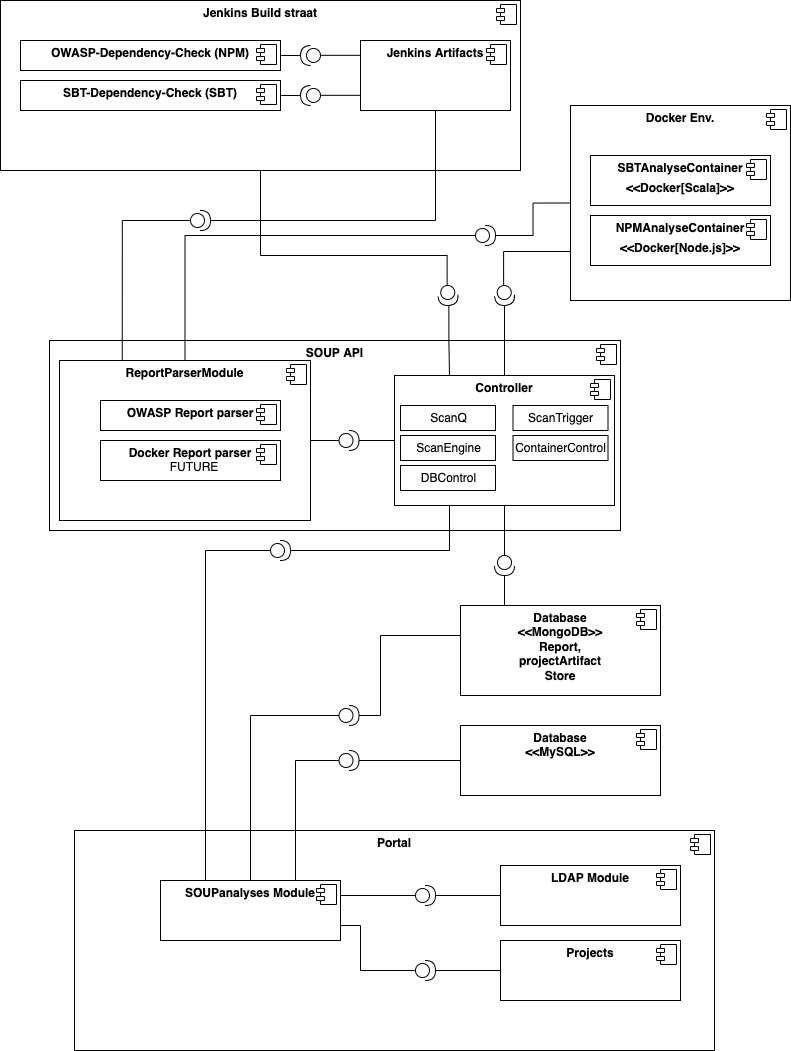
\includegraphics[width=10cm]{gfx/UMLcomponentDiagram}
%    \caption{Componenten SOUP Analyse Systeem}
%    \label{fig:SOUP-Components}
%\end{figure}
\section{Datamodel}\label{subsec:intern-datamodel}
De data die de drie services gebuikten is opgesteld in een intern datamodel dat in figuur~\ref{fig:SOUP-SoupApiDm} is te zien In het datamodel zijn voorzieningen waarin per module een analyse op geslagen kan worden waarin vervolgens de in die module op het moment van de analyse aanwezige dependencies met de bekende kwetsbaarheden op kunnen worden geslagen.
\begin{figure}[H]
    \myfloatalign
    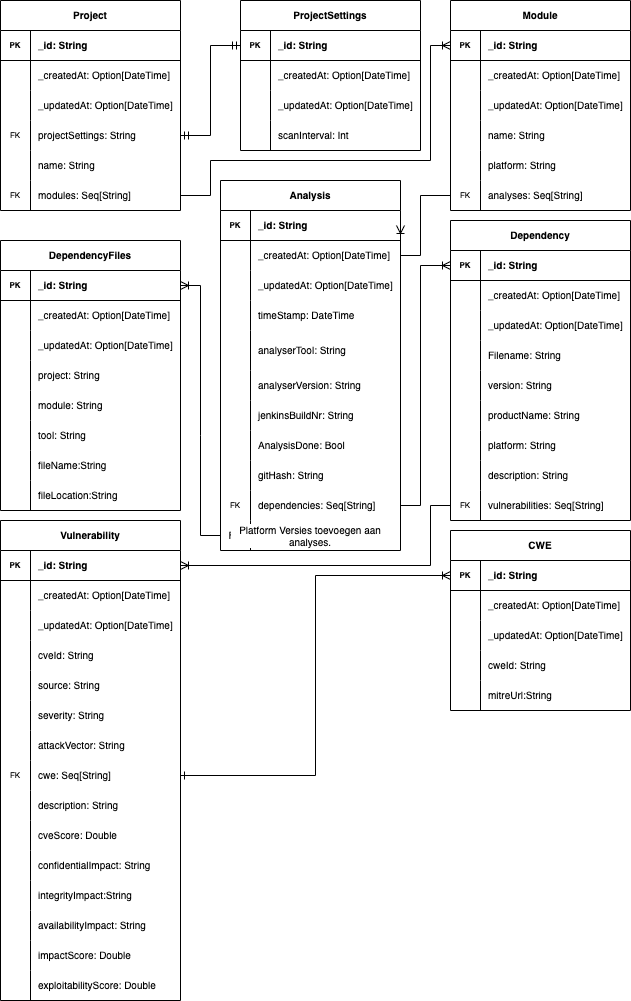
\includegraphics[width=12cm]{gfx/SOUPAPI-SOUPAPI DM}
    \caption{Intern Datamodel}
    \label{fig:SOUP-SoupApiDm}
\end{figure}
%TODO checken of 8pt leesbaar is op print
%TODO tekst beter structureren

Eaglescience werkt op projectbasis, waarbij één of meer modulen de applicatie vormen. Deze worden dan ook in project opgeslagen naast de naam van het project en projectSettings welke gebruikt worden door de SOUPAPI om te fungeren. Onder projectsettings staat nu een scanInterval die ingesteld kan worden in een aantal dagen dat er tussen de analyses mag zitten. ProjectSettings is bewust apart genomen omdat dit de ruimte bied om de toekomst benodigde instellingen toe tevoegen.

Voor de module wordt de naam en het platform waarin het geschreven is opgeslagen. Aan de de modulen worden de analyses gehangen. Analyses worden gedaan op moduleniveau en niey op projectniveau. Dit geeft de mogelijkheid om de modulen los van elkaar te kunnen analyseren en hier de data van op te slaan.

In de analsyses wordt de timestamp opgeslagen om te achterhalen wanneer deze is uitgevoerd. Als ook het buildnummer uit jenkins als deze is uitgevoerd binnen de jenkins timeline. Ook wordt de githash opgeslagen om op die manier te kunnen achterhalen welke commit er geanalyseerd is.

De analyses bevat een lijst met dependencies die in de modules voorkomen. Voor deze dependencies worden de filenaam, versie, productnaam, en platform opgeslagen. Als ook een descriptie als deze wordt meegegeven door de SCA Tool. Als de dependency een Vulnerability beavt wordt deze aan de dependency toegevoegd. de Vulnerability bevat impactscores voor confidentiality, integrity en availability als een algehele impact score. Ook wordt de CWE opgeslagen waarin het id en de url naar meer informatie wordt opgeslagen.

Op het moment dat een analyse is uitgevoerd in de Jenkins pipeline worden ook de files waarin de dependency declaraties staan op geslagen per Analyse. Deze dependency files kunnen op een later moment worden gebruikt om een analyse uit te voeren voor een project of module.

\section{Dev-stack}

Om de applicatie te kunnen ontwikkelen is er voor de volgende dev-stack gekozen.

De SOUPAPI, backend van de server worden geschreven in Scala met het PlayFramework als webapplicatieFramework. De frontend van de portal wordt geschreven in Angular 13 omdat dit op dit moment ook wordt gebruikt voor de ontwikkeling van diezelfde portal en er is geen reden om dit te veranderen.
De keuze voor Scala met playframework en Angular lig voor de hand omdat dit al bekend is binnen de dev-stack van eaglescience.

De SOUP API zelf wordt in een docker container gedraaid.

